\chapter{Discussion}
\label{chap:discussion}

Thematically analysing the interviews revealed several common perceptions of the participants and allowed for structuring the research's findings as described in Section~\ref{chap:findings}. Furthermore, it left room for interpreting and relating them on a larger scale. The following diagrams integrate all findings and generate a common view towards information and communication challenges, benefits and improvements. They lay the foundation for a set of trade-offs around \ac{XFT} empowerment and their workflow and the overarching organisation. These trade-offs in turn can impact the productivity of \acp{XFT} positively or negatively.

\section{Communication \& Information}

As outlined in the~\nameref{chap:findings}, the analysis of the interviews' transcriptions revealed that respondents elaborate on information and communication by mentioning associated challenges, benefits and possible improvements. 

\begin{figure}[h!]
  \centering
  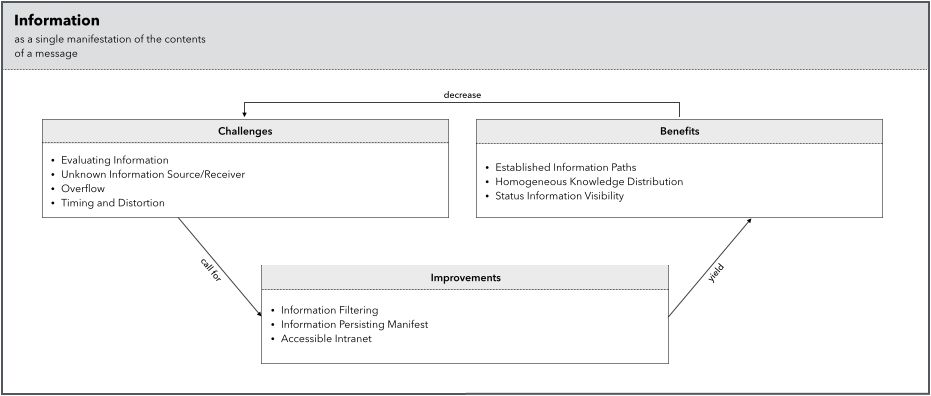
\includegraphics[width=0.98\textwidth]{figures/information.png}
  \caption{Information challenges, benefits and improvements}
  \label{fig:information}
\end{figure}

In addition, all three elements show an equal relation among one another within the fields of information and communication. Targeted benefits can only be realised by addressing a known challenge with a tailored improvement. As outlined in Figures~\ref{fig:information} and~\ref{fig:communication}, challenges can be overcome by applying an improvement, which in turn \emph{decreases} the challenge but might also strengthen another one as a negative side effect. Side effects are caused by the tendency of improvements to change the nature of communication and information. After all, this might just affect other existing challenges or can even create new ones.
In general, challenges \emph{call for} improvements while the improvement itself \emph{yields} certain benefits. It is important to note that one can not overcome a challenge without addressing it with a concrete improvement.

\begin{figure}[h!]
  \centering
  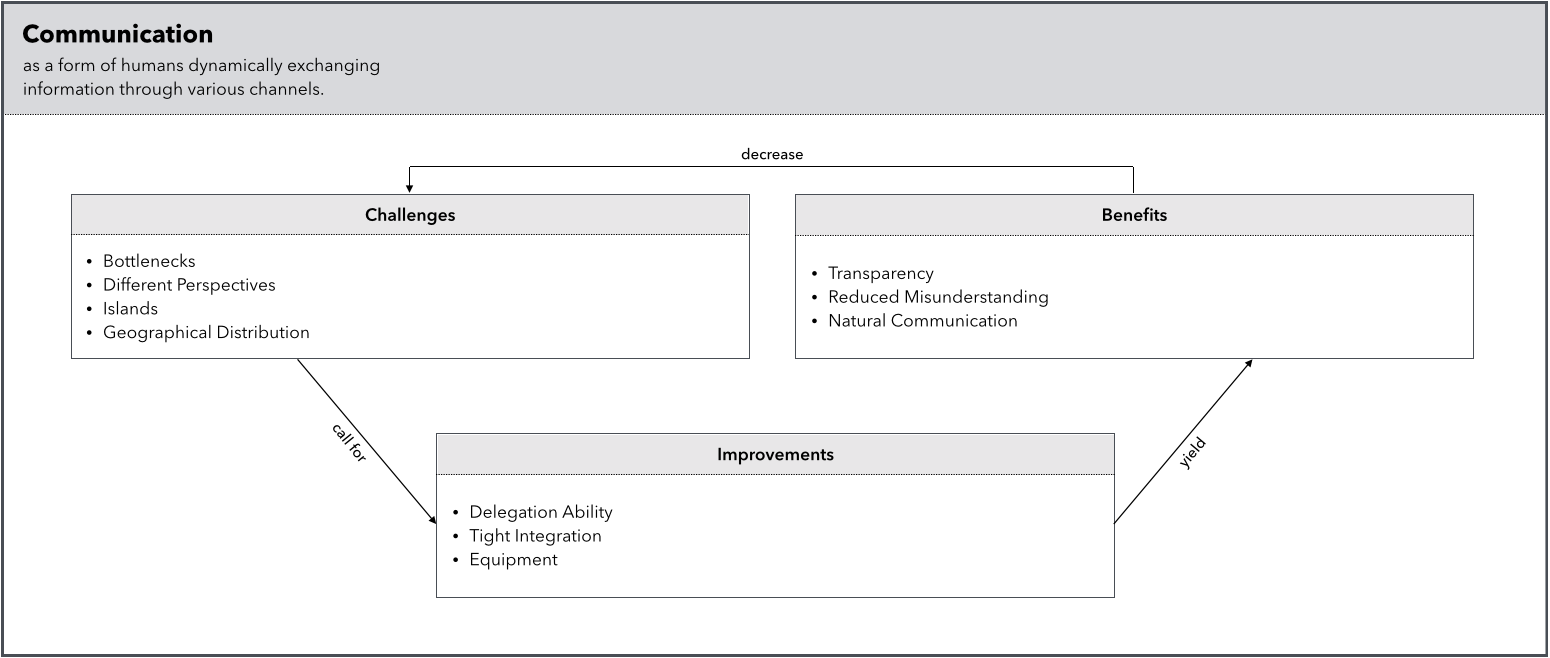
\includegraphics[width=0.98\textwidth]{figures/communication.png}
  \caption{Communication challenges, benefits and improvements}
  \label{fig:communication}
\end{figure}

Figure~\ref{fig:theming-diagram} illustrates the overall relation with a presence of \emph{mutual influence} between communication and information. Whenever the way in which communication is dynamically carried out is changed, it can also feedback into information and affect its challenges and possible benefits.~\citet{pikkarainen2008impactagilecommunication}, for instance, call the increasing amount of informal communication evolving into an inevitable challenge for large-scale agile organisations. The studied organisation and its~\acp{XFT} declare the rising \emph{information overflow} as one of the main challenges which should be addressed with a variety of improvements such as an ability for \emph{information filtering} and an \emph{accessible intranet}. The found communication challenge of having \emph{different perspectives} towards the level of details on a certain topic or compulsory collective meetings varying in benefit for its participants is partially caused by the new and often uneven distribution of responsibilities in the process of empowering the \acp{XFT}. This growing disconnection between units within the organisation and its relation to empowerment has also been pointed out previously~\citep{millslimitsempowerment, tessemindividualempoqerment}.

Furthermore, the \emph{dynamic nature} of communication itself promotes this \emph{mutual} relationship in which information is defined as a \emph{manifestation of the contents of a message}.\\
In the context of an organisation, properties of information feed into communication and vice versa. One side of this \emph{mutual influence} manifests itself whenever information is exchanged by communicating. Communication success depends on the present information challenges. Communication is likely to be efficient whenever sources are accessible without an overflow, correct information has been evaluated, the piece of information is not distorted and appropriate receivers are known. \emph{Communication islands} for instance, according to~\citet{kettunen2008agileorg}, often arise from the accumulation of knowledge — an issue to which this study additionally observed that islands can develop unintentionally. A later attempt to eliminate islands by publicly offering the gathered knowledge often results in an excessive demand of knowledge sharing for its members having a distractive effect on their work focus. \emph{Bottlenecks} and \emph{islands} have also been identified by~\citet{curtis1988fieldstudysoftwaredesign}. They are caused by communication paths being hard to establish and an inability to make decisions without clear responsibilities in place. Still, the importance of informal communication is highlighted. Issues arise as soon as a high level of informal communication has to integrate within various chains of command or has to take place with roles far out of the natural communication environment~\citep{curtis1988fieldstudysoftwaredesign}.

Similarly, the other way around, the state of information with its associated challenges and benefits is also influenced by communication. Information challenges tend to arise by changing communication procedures and adjustments of the organisational context. A shift towards more geographical distribution, for instance, generates new communication challenges which yet again render new information demands and requirements. This is also stated by~\citet{kraut1995coordinationinsd}, who emphasize the geographical distance as a negative influence to communication behaviour. 

\section{Trade-offs \& Productivity Determinants}

Both distinct but interdependent fields of information and communication then influence a set of trade-offs through setting up the basis of organisation's position in relation to being rather \emph{transparent} or focussing on \emph{islands}.

Figure~\ref{fig:trade-offs} illustrates different trade-offs which are greatly influenced by the described interplay of communication and information, its challenges and benefits:

\begin{description}
   \item[Organisation:] Islands vs Transparent
   \item[XFT Empowerment:] Responsibility Specialised vs. Responsibility Broadened
   \item[XFT Workflow:] Static vs. Emergent
\end{description}

All three trade-offs contain the rather agile perceptions towards organisations, workflow and empowerment on their right extreme. Their left extreme outlines the more traditional perceptions towards software development processes. None of the two is to be understood as generally beneficial as their value depends on the context and its requirements.

\begin{figure}[h!]
  \centering
  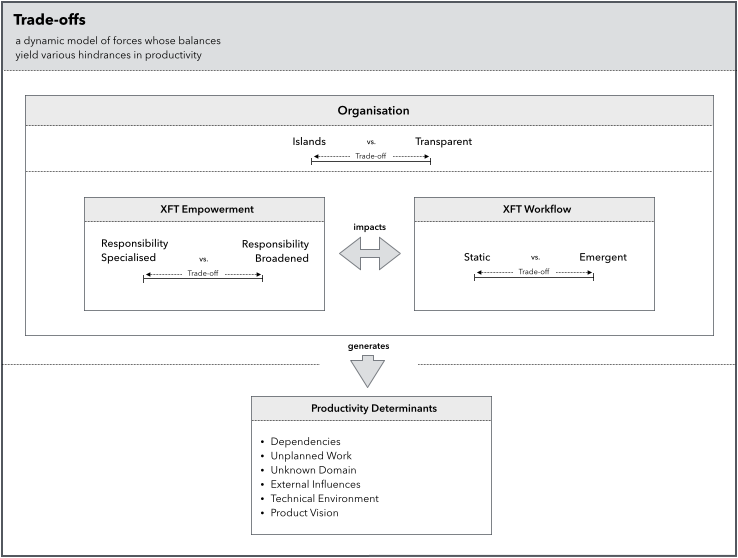
\includegraphics[width=0.98\textwidth]{figures/tradeoffs.png}
  \caption{Trade-offs in empowerment, workflow and organisational influence}
  \label{fig:trade-offs}
\end{figure}

Interviewees noted these previously mentioned concepts touching on communication and information mostly in the context of the present organisational structure as outlined in Figure~\ref{fig:org-structure}. Additional to the organisational structure, interviewees interact with organisational aspects such as processes definitions and prevailing roles definitions. 
In an agile organisation these elements are usually aligned with the organisation's intention towards being \emph{transparent} or favouring \emph{islands} (see Figure~\ref{fig:trade-offs}).
Single decisions within a given organisational framework by changing processes or just carrying out work can then change the positioning on the organisational trade-off in one of its directions, while neither one of the two extremes are wished for under all circumstances. \emph{Transparency} may seem to always be desirable to allow for a fluent information circulation but bears issues at large scale causing confusion by overflow paralysing decision making. Forming \emph{islands} may appear negatively connotated as it disconnects individual units but is advantageous in efficiency for isolated and specialised tasks.

The trade-off on a level of an organisation envisioning the adoption of agile methodologies influences two subordinate trade-offs: one around the \ac{XFT} empowerment and the second around their workflow. The \ac{XFT} empowerment bears a necessary decision on how responsibilities should be delegated towards teams. On the one hand, an \ac{XFT}'s responsibilities can be \emph{specialised} according to a product or its members' competences. On the other hand, various degrees of \emph{broadened} responsibilities can be assigned. Completely \emph{broadened} \acp{XFT} would therefore be able to take over almost any task and solve most impediments within their environment without much external guidance. The empowerment approach tends to have negative side effects on both extremes. Assigning too many responsibilities is a cause of \acp{XFT} being overwhelmed and loosing focus. On the contrary, highly \emph{specialised} teams would strive in a well-defined field with a preferably narrow scope. Context changes or various external dependencies can break their focus and turn out costly for their efficiency.

Software development also entails a workflow in which a trade-off between an \emph{emergent} and \emph{static} nature should be made. An \emph{emergent} workflow is composed of groups solving a task self-coordinated without dedicated supervision. Whereas groups working in a \emph{static} fashion tend to require more oversight and are more suited for the assignment of predefined tasks. An \emph{emergent} workflow reduces the need for pre-planning but tends to struggle with carrying out tasks of higher complexity with too many interdependencies. \emph{Static} workflows, through their static structure, are more compatible with a vast amount of dependencies but are vulnerable by their need of coordination and supervision.

The three mentioned trade-offs around the \emph{organisation}, \emph{empowerment} and \emph{workflow} mutually influence one another. The alignment within one trade-off can ease reaching a certain position on another but might be hindered by the third. The possibility to freely adjust a trade-off might thereby not always be there unless others are changed previously. This strong attachment is also noticeable by certain incompatibilities between the trade-offs' positions. An \emph{emergent} workflow, for instance, is difficult in an organisation favouring \emph{islands} and a \emph{specialised} strategy towards empowerment. \emph{Broad} \acp{XFT} prefer some level of \emph{transparency} with a rather \emph{emergent} workflow to engage in solving changing tasks. 

Finally, settling on all trade-offs defines a set of dependent \emph{productivity determinants}. The existence of these concrete determinants and their severity is influenced by the mentioned trade-offs and the organisation's nature. The often negative effect of \emph{technical dependencies} and associated challenges potentially creating domino effect or even vicious circle have previously been pointed out by~\citet{nelson2013technicaldependencies}. Concerns regarding planning and maintaining a shared \emph{product vision} have also been mentioned~\citep{badampudi2013proddelay}. Still,~\citet{badampudi2013proddelay} state that these are less rooted in the agile's need to flexibility but rather caused by unclear requirements, false customer collaboration and a lack of competence. 

The key is to identify acceptable \emph{productivity determinants} while moving along information and communication challenges and the adjustment of all trade-offs until the intended determinants carry into effect. The trade-offs are just means to an end and agility lies in the ability to adapt and chose the most suitable constellation under given circumstances and an intended outcome.
